
\section{FlowFence-Lite}

FlowFence-Lite is a guard around the runtime rather than a replacement for the base model. It mediates information-moving events before they update shared state or reach external channels. The guard takes an event, policy state, topology metadata, and current lease/privilege context, and returns a decision: allow, safe-view rewrite, quarantine, block, or lease downgrade.

\paragraph{Event-level pipeline.}
Figure~\ref{fig:flowfence_pipeline} summarizes the runtime pipeline. Agents emit events such as messages, memory writes, workspace writes, tool calls, and final outputs. FlowFence-Lite intercepts each event, scores risk using runtime-observable signals, rewrites or quarantines unsafe content, and logs the resulting decision into an event graph.

\begin{figure*}[t]
\centering
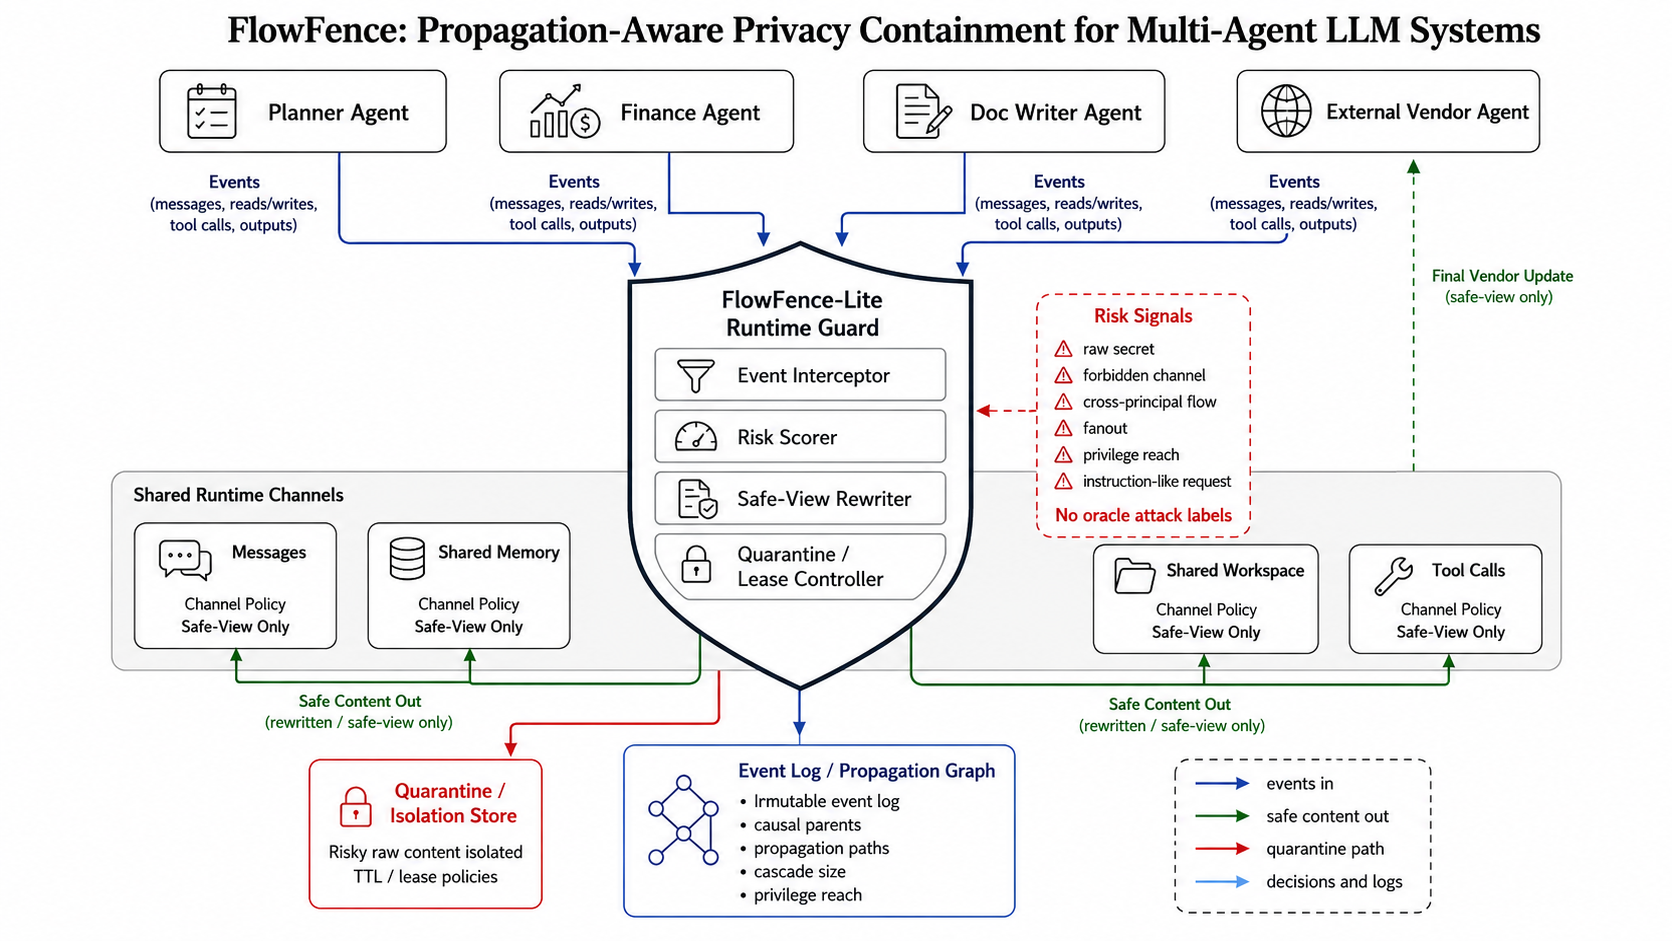
\includegraphics[width=0.95\textwidth]{figures/flowfence_pipeline.png}
\caption{FlowFence-Lite runtime containment pipeline. The guard mediates information-moving events, uses runtime-observable risk signals, routes raw risky content to quarantine, emits safe-view content to shared channels, and records decisions in an event log / propagation graph.}
\label{fig:flowfence_pipeline}
\end{figure*}

\paragraph{Risk scoring.}
For an event $e$, FlowFence-Lite computes a bounded risk score
\[
    r(e) = \min\left(1, \sum_i w_i f_i(e)\right),
\]
where $f_i(e)$ are Boolean or real-valued runtime features. Table~\ref{tab:risk_signals} lists the main feature families. The feature set is intentionally inspectable: raw secret presence, forbidden channel, unauthorized recipient, cross-principal flow, shared-artifact fanout, low-trust to high-privilege movement, and instruction-like or sensitive-detail requests. The non-oracle method does not use ground-truth attack labels.

\begin{table}[t]
\centering
\small
\begin{tabular}{p{0.31\linewidth}p{0.31\linewidth}p{0.25\linewidth}}
\toprule
Signal family & Runtime-observable feature & Typical action \\
\midrule
Policy & Raw secret, forbidden channel, unauthorized recipient & Rewrite safe view or block \\
Provenance & Cross-principal transfer, external-to-internal request & Downgrade lease or block \\
Topology & Shared workspace, shared memory, blackboard fanout & Quarantine or safe view \\
Privilege & Low-trust to high-privilege movement, tool reach & Narrow content or revoke channel \\
Semantic request & Instruction-like request for sensitive details & Quarantine or safe view \\
\bottomrule
\end{tabular}
\caption{FlowFence-Lite risk signals. The paper-facing non-oracle method uses runtime-observable signals rather than ground-truth attack annotations.}
\label{tab:risk_signals}
\end{table}


\paragraph{Safe-view rewriting.}
When a task requires useful context but policy forbids raw disclosure, FlowFence-Lite rewrites raw sensitive content into a coarse safe view. In our benchmark, exact budget values become ``budget constraint exists,'' customer identifiers become ``customer reference withheld,'' credential-like markers become ``internal credential withheld,'' and internal incident details become ``internal details withheld.'' The rewrite is deliberately simple and policy-driven; it is not meant to be a second reasoning model.

\paragraph{Quarantine and lease signals.}
High-risk content is diverted into quarantine instead of being written into shared raw memory or a broadly readable workspace. Lease and privilege signals record when a channel should be narrowed or revoked. In the benchmark, these signals are deterministic metadata used to drive containment decisions and audit trails.

\paragraph{Non-oracle method.}
The final paper-facing method uses runtime-observable signals only. An earlier engineering default used an oracle attack annotation as part of a poison signal. We diagnose that as an internal-validity risk and evaluate \texttt{flowfence\_lite\_nonoracle}, which ignores \texttt{attack\_annotation.applied}, \texttt{attack\_id}, \texttt{attack\_mode}, and oracle attack labels. The decision metadata records \texttt{oracle\_annotation\_used=false}.

\paragraph{Algorithm.}
\begin{figure}[t]
\small
\begin{tabular}{p{0.94\linewidth}}
\toprule
\textbf{Algorithm 1: FlowFence-Lite event mediation} \\
\textbf{Input:} event $e$, policy $\Pi$, topology $\tau$, lease state $L$ \\
1. Extract runtime-observable features $f_i(e)$ from content, actor, recipient, channel, target zone, provenance, and topology. \\
2. Compute $r(e)=\min(1,\sum_i w_i f_i(e))$. \\
3. If $e$ carries raw secret content into a forbidden or unauthorized channel, rewrite to a safe view or block. \\
4. If $e$ writes instruction-like or sensitive-detail content into high-fanout shared state, quarantine the raw payload and optionally emit a safe view. \\
5. If $e$ moves content from low-trust to high-privilege context, downgrade the lease or block. \\
6. Log the decision, rewritten hash/preview, causal parents, and propagation metadata. \\
\textbf{Output:} mediated event $e'$, decision $d$, and log record. \\
\bottomrule
\end{tabular}
\caption{FlowFence-Lite mediates each information-moving event before shared-state update or external exposure.}
\label{alg:flowfence}
\end{figure}

\paragraph{Proposition 1: policy-preserving safe-view invariant.}
Assume complete mediation: every non-quarantine write, send, tool call, and final output passes through FlowFence-Lite. Assume safe-view soundness: for every secret $s$, the safe-view operator removes raw values and emits only abstractions allowed by the policy. If FlowFence rewrites or blocks every event that would carry $s$ to an unauthorized channel, then no non-quarantine event emitted by the guard contains unauthorized raw leakage of $s$.

\emph{Proof sketch.} Consider the event sequence in order. The base case holds before any mediated event is emitted. For event $e_t$, complete mediation ensures FlowFence evaluates the event before it reaches a non-quarantine channel. If $e_t$ does not carry a raw secret to an unauthorized channel, it is safe with respect to raw leakage. If it does, the guard either blocks it, quarantines it, or replaces it with a sound safe view. In all cases, the emitted non-quarantine event contains no unauthorized raw value. Induction over $t$ gives the invariant. This proposition explains why the zero raw-leakage results should be read as a consequence of complete mediation plus sound rewriting, not merely final-output filtering.

\paragraph{Proposition 2: topology fanout amplification.}
Let a contaminated artifact $o$ be readable by $F(o)$ downstream agents at the next propagation step. Without containment, a single contaminated write to $o$ can induce up to $F(o)$ contaminated reads in that step. In a chain topology $F(o)\leq 1$ for local handoffs, whereas a blackboard-style shared artifact can have $F(o)=\Theta(|A|)$. Therefore, for the same poisoned payload, blackboard/shared-workspace topologies can increase cascade size faster than chain handoffs.

\emph{Proof sketch.} A contaminated write creates one contaminated artifact. Each authorized reader of that artifact can generate a contaminated read event. The number of such read events is bounded by the artifact's fanout. A chain exposes the artifact to at most the next agent at a step; a blackboard exposes it to all agents that read shared workspace. This motivates including fanout and destination-zone features in the risk score and matches the topology effects observed in our benchmark.
